\documentclass[9pt,twocolumn,twoside]{pnas-new}
% Use the lineno option to display guide line numbers if required.
% Note that the use of elements such as single-column equations
% may affect the guide line number alignment. 

\templatetype{pnasresearcharticle} % Choose template 
% {pnasresearcharticle} = Template for a two-column research article
% {pnasmathematics} = Template for a one-column mathematics article
% {pnasinvited} = Template for a PNAS invited submission

\usepackage{pslatex}
\usepackage{amsfonts}
\usepackage{graphicx}
\usepackage{color}
\usepackage{todonotes}
\usepackage{dsfont}
\usepackage{array}
\usepackage{textcomp}
\usepackage{multirow}
\usepackage{subfig}
\usepackage{trackchanges}
% trackchanges commands:
%   \note[editor]{The note} 
% \annote[editor]{Text to annotate}{The note} 
%    \add[editor]{Text to add} 
% \remove[editor]{Text to remove} 
% \change[editor]{Text to remove}{Text to add}


\title{Contextual flexibility in visual communication}

% Use letters for affiliations, numbers to show equal authorship (if applicable) and to indicate the corresponding author
% \author[Author Names]
% {Judith E. Fan \affil{1,*}, Robert X.D. Hawkins \affil{1,*}, Mike Wu \affil{2}, \and Noah D. Goodman \affil{1,2}}

% \affiliation{1}{Department of Psychology, Stanford University, Stanford, CA 94305}
% \affiliation{2}{Department of Computer Science, Stanford University, Stanford, CA 94305}
% \affiliation{*}{These authors contributed equally to this work.}

% \correspondingauthor{Judith E. Fan}{jefan@stanford.edu}

\author[a,1,*]{Judith E. Fan}
\author[a,*]{Robert X.D. Hawkins} 
\author[b]{Mike Wu}
\author[a,b]{Noah D. Goodman}

\affil[a]{Department of Psychology, Stanford University}
\affil[b]{Department of Computer Science, Stanford University}
\affil[*]{These authors contributed equally to this work.}

% Please give the surname of the lead author for the running footer
\leadauthor{Fan} 

% TODO: Currently a bit too long (and probably too in the weeds...) 
\significancestatement{}

% Please include corresponding author, author contribution and author declaration information
\authorcontributions{Please provide details of author contributions here.}
\authordeclaration{Please declare any conflict of interest here.}
\correspondingauthor{\textsuperscript{1}To whom correspondence should be addressed. E-mail: author.two\@email.com}

% Keywords are not mandatory, but authors are strongly encouraged to provide them. If provided, please include two to five keywords, separated by the pipe symbol, e.g:
\keywords{drawing $|$ deep learning $|$ pragmatics $|$ computational modeling $|$ Rational Speech Act framework}

\begin{abstract}
Communication is central to the success of our species: it allows us to learn from each other, coordinate our actions, and express otherwise hidden thoughts. Critically, human communication goes beyond language production --- humans also express their ideas in visual form. Visual communication lies at the heart of key innovations, and forms the foundation for the cultural transmission of knowledge and higher-level reasoning. This paper examines drawing, the most basic form of visual communication. Communicative uses of drawing pose a core challenge for theories of vision and communication alike: they require a detailed understanding of how sensory information is encoded and how social context guides what information is relevant to communicate. Our computational modeling approach addresses this challenge by combining a high-performing computational model of vision with a formal Bayesian model of social reasoning during communication in order to explain how people flexibly adapt their drawings according to the current context. We employ drawing-based reference games throughout our modeling and experimental work. These reference games involve two players: a \textit{sketcher} who aims to help a \textit{viewer} pick out a target object from an array of alternative, distractor objects by representing it in a drawing. We found that people exploit information in common ground with their partner to efficiently communicate, and that this contextual flexibility was well explained by our computational model. In the long run, understanding the computational basis of visual communication may shed light on the nature of human visual abstraction and the emergence of graphical conventions.
\end{abstract}

\dates{This manuscript was compiled on \today}
\doi{\url{www.pnas.org/cgi/doi/10.1073/pnas.XXXXXXXXXX}}

\begin{document}

% Communication is not limited to verbal language; humans can make use of many different tools to convey meaning to a partner. While theories of communication often rely upon the existence of modality-general pragmatic reasoning mechanisms, these predictions have rarely been tested outside the verbal modality. In this experiment, we aim to test how context -- the set of potential referents in common ground -- affects visual communication: using drawings to convey the identity of rich naturalistic images. Past work in the verbal modality has shown a strong influence of speaker informativity: when the intended referent is surrounded by very similar objects, speakers send more detailed and verbose messages to help the listener distinguish it. We expect analogous results to hold in the visual modality. For instance, when referring to a car in a context containing dogs and birds, speakers should use simpler, more abstract drawings than when referring to the same object in the context of other cars.


% Optional adjustment to line up main text (after abstract) of first page with line numbers, when using both lineno and twocolumn options.
% You should only change this length when you've finalised the article contents.
\verticaladjustment{-2pt}

\maketitle
\thispagestyle{firststyle}
\ifthenelse{\boolean{shortarticle}}{\ifthenelse{\boolean{singlecolumn}}{\abscontentformatted}{\abscontent}}{}

% high level
Communication is central to the success of our species: it allows us to learn from each other, coordinate our actions, and express otherwise hidden thoughts. Critically, human communication goes beyond language production --- humans also express their ideas in visual form. Visual communication lies at the heart of key innovations, and forms the foundation for the cultural transmission of knowledge and higher-level reasoning. Drawing is perhaps the most direct and basic form of visual communication. We perceive drawings of objects as resembling physical objects in spite of the fact that drawings and objects are profoundly different in composition.

In the appropriate context, even a few strokes can express the identity of a face \cite[]{bergmann2013impact}, a suggested route \cite[]{agrawala2001rendering}, or an intention to act \cite[]{Galantucci:2005uh}. Conventionalized representations such as maps, graphs, and diagrams can transmit high-dimensional data and convey complex ideas by recombining relatively few geometric primitives, such as boxes, lines, arrows, ellipses \cite[]{tversky2000lines}. Despite the ubiquity and importance of such visualizations, we lack a unified computational theory of how human perception, action, and social inference are integrated to support flexible visual communication.

Communicative uses of drawing pose a core challenge for theories of vision and communication alike: they require a detailed understanding of how sensory information is encoded, how social context guides what information is relevant to communicate, and estimating the costs of visual production. In this paper, we meet this challenge by combining high-performing models of sensory representation from deep learning with insights from Bayesian cognitive models of social reasoning in language. 

There is now abundant and converging evidence that deep convolutional neural networks (DCNNs) optimized to recognize objects in natural photographs can learn general-purpose feature representations that support a wide variety of visual tasks, including but not limited to object categorization, segmentation, and pose/size estimation \cite[]{hong2016explicit,he2017mask}.

% recent successes learning general visual features, but these inherently acontextual
In particular, despite the fact that drawings are highly abstracted away from natural visual inputs, a relatively modest amount of `fine-tuning' of models previously trained only on photos has been shown to lead to human-level performance on sketch categorization \cite[]{yu2015sketch}, as well as vast improvements in discerning image-level correspondences between sketches and photos \cite[]{sangkloy2016sketchy}. Even without fine-tuning, prior work has shown a striking isomorphism in the representations of object categories in drawings and photos at higher layers in these models \cite[]{fan2015common}. As such, models from this architecture class are a strong candidate for an encoder that can support the level visual abstraction required for representing abstract information in drawings.

However, these visual feature representations are inherently acontextual, and cannot explain why people might use one drawing to communicate an idea in one context (e.g., XX), and a different drawing in another context (e.g., XX). Rational Speech Act (RSA) models provide a probabilistic framework for deriving communicative flexibility from general principles of social cognition \cite{GoodmanFrank16_RSATiCS}.  

These models draw on ideas and insights from decision theory, probabilistic models of cognition, bounded rationality, and linguistics, taking particular inspiration from the insights of Paul Grice (\citeyear{grice1975syntax}), who provided a philosophical framework for understanding how natural language use reflects social reasoning in context. Gricean listeners assume speakers are cooperative, choosing appropriately informative utterances to convey particular meanings. Under this assumption, listeners attempt to infer the speaker's intended communicative goal, working backwards from the form of the utterance. RSA models formalizing this core idea in terms of Bayesian inference have provided unified explanations for a variety of complex linguistic patterns, achieved good quantitative fits with experimental data, and been incorporated into artificial agents that communicate with each other to solve real-world tasks.

Previous work has shown that RSA models account for context sensitivity in human speakers \cite[]{GrafEtAl16_BasicLevel}. 

% For instance, if a speaker needs to refer to a Dalmatian that appears alongside a poodle and a bear, the model predicts that this speaker will prefer the more specific utterance (``Dalmatian'') to the shorter and lower-cost basic-level utterance (``dog''). This is because the literal meaning of the word ``dog'' fits both the Dalmatian and poodle, whereas the word ``Dalmatian'' only fits the Dalmatian. Consequently, the speaker model reasons that ``Dalmatian'' is more informative. By using the word ``Dalmatian'', the speaker encourages the listener to infer the single correct world state (i.e., the target is the Dalmatian) instead of allowing two world states to seem probable, one of which is incorrect (i.e., the target is the poodle). In a context where there is only one dog, however, the speaker will prefer to say ``dog'', which is as informative as ``Dalmatian'' but is less costly to produce. 

\section*{Methods}

\subsection*{Participants}

A total of 192 unique participants, who were recruited via Amazon Mechanical Turk (AMT) and grouped into pairs, completed the experiment. 

\subsection*{Stimuli}

Stimuli were 32 3D mesh models of objects belonging to 4 categories (i.e., birds, chairs, cars, dogs), containing eight objects each. 40 color images of each object were produced by rendering it from a 10$^{\circ}$ viewing angle (i.e., slightly above) at a fixed distance on a gray background, each rotated by an additional 9$^{\circ}$ about the vertical axis. 

\subsection*{Task}

Drawings were collected in the context of an online, sketching-based reference game (``Guess My Sketch!''). The game involved two players: a \textit{sketcher} who aims to help a \textit{viewer} pick out a target object from a set of distractor objects by representing it in a sketch. On each trial, both participants were shown an array of the same four objects; however, the positions of these objects were randomized for each participant. On each trial, one of the four objects was highlighted on the sketcher's screen to designate it as the target. 

Sketchers drew using black ink on digital canvas (pen width = 5 pixels; 300 x 300 pixels) embedded in a web browser window using Paper.js (http://paperjs.org/). Participants drew using the mouse cursor, and were not able to delete previous strokes. Each stroke of which was rendered on the viewer's screen immediately upon the completion of each stroke. There were no restrictions on how long participants could take to make their drawings. After clicking a submit button, the viewer guessed the identity of the drawn object by clicking one of the four objects in the array. Otherwise, the viewer had no other means of communicating with the sketcher. Both participants received immediate task-related feedback: the sketcher learned which object the viewer had clicked, and the viewer learned the identity of the target. Both participants earned bonus points for each correct response. 

For each pair, objects were grouped into eight quartets: Four of these quartets contained objects from the same category (``close''); the other four of these quartets contained objects from different categories (``far'' condition). Each quartet was presented four times, such that each object in the quartet served as the target exactly once. The assignment of objects to quartet and condition was randomized across pairs. 

\subsection*{Modeling}

\subsubsection*{Visual encoder module}

Features were extracted using VGG-19 \cite{simonyan2014very}, a high-performing deep convolutional neural network model architecture that had been pretrained to categorize objects on the Imagenet database, which contains millions of photographs from hundreds of object categories \cite{deng2009imagenet}. Despite the fact that drawings are highly abstracted away from natural visual inputs, prior work has shown a striking isomorphism in the similarity structure \cite{kriegeskorte2008matching} of object categories in drawings and photos at higher layers in these models \cite[]{fan2015common}, without any additional training.

While these models excel at (and were indeed optimized for) categorization of objects, two additional competencies are required to succeed at the visual communication task described above.

First, an observer must be able to represent fine-grained relationships between different images of objects from the same category; second, this observer must also be able to discern image-level correspondences between drawings and photos of the same object. 

In order to better approximate the granularity with which human observers can distinguish different images, we augment VGG19 with a smaller \textit{adaptor} network that learns a common feature representation for drawings and photos. 

This approach has been successfully used in prior work to better predict human semantic categorization judgments \cite{peterson2016adapting}, and to improve sketch-based image retrieval \cite[]{sangkloy2016sketchy}. 


\subsubsection*{Social inference module}

To instantiate communicative flexibility in context, we generalize the Rational Speech Act (RSA) modeling framework, originally developed for linguistic communication. At the core of the RSA framework, as applied to linguistic communication, is the Gricean proposal that speakers aim to produce utterances that are concise yet informative. We adapt this proposal to visual communication by assuming that sketchers also aim to produce drawings that are both simple and informative. 

Formally, the sketcher, $\mathcal{S}$, is a decision-theoretic agent who produces drawings, $d$, by (soft) maximizing their utility function, $U$, given a particular object referent, $o$: 

\begin{equation}
\mathcal{S}(d|o) \propto e^{\alpha U(d,o)}
\end{equation}

Here, $\alpha$ is a softmax parameter. As $\alpha \rightarrow \infty$, the sketcher approaches the optimal maximizing policy. 

The sketcher's utility function, $U$, trades off the extent to which the drawing is informative to the viewer, $\mathcal{V}$, and the cost of producing the drawing, $C(d)$. This notion of informativity is defined by the (natural log) probability that a viewer would select the true object referent given the drawing and current context:

\begin{equation} \label{sketcher_utility}
U(d, o) = \ln \mathcal{V}(o|d) - C(d)
\end{equation}

This sketcher $\mathcal{S}$ is \emph{pragmatic} because they evaluate informativity by considering rational viewer agent ($\mathcal{V}$) who assigns a score to the correspondence between the drawing and each object that is proportional to the perceptual similarity, $P$, between the drawing and each potential object referent in context:

\begin{equation} \label{literal_viewer_score}
\mathcal{V}(o|d) \propto P_{o,d}
\end{equation}

To compute these perceptual similarity scores, the sketcher agent (who can also view the sketch and objects) extracts a feature vector representation from each of the target and distractor objects using the fixed visual encoder, and computes the distances between each of these vectors and the potential sketches it could produce. 

This has the effect of biasing the model to depict properties of the target object that distinguish it from the distractors, while also preferring sketches that are less costly to produce, $C(d)$, i.e., requiring fewer strokes or less ink.


\section*{Results}

\subsection*{Task performance}

If sketchers aim to make their sketches informative without being too costly to produce, they will modulate the level of detail in their drawings according to the set of alternative hypotheses under consideration by the viewer. For instance, in the \textit{close} condition where the target and distractors belong to the same basic-level category, sketchers should make detailed drawings to highlight fine-grained distinctions, even though this requires including additional detail. By contrast, in the \textit{far} condition where the target and distractors belong to different basic-level categories, the sketcher can afford to produce simpler drawings by omitting excess detail.

Consistent with this prediction, we found that sketchers applied fewer strokes (close = 8.03, far = 13.5, \textit{p} $<$ 0.001), used less ink (measured by proportion of the canvas marked: close = 0.054, far = 0.042, \textit{p} $<$ 0.001) and spent less time (close = 30.3s, far = 13.7s, \textit{p} $<$ 0.001) to make their drawings in the far condition than in the close condition. 

Despite the relative sparsity of drawings produced on far trials, viewers were close to ceiling on inferring the target (99.7\%). Performance was also high on close trials (87.7\%), even though this required that people discriminate the correspondence between a sketch and its referent in the context of highly similar distractors. 

\subsection*{Modeling}


\subsubsection*{Code availability} The code for the analyses presented in this article is publicly available in a Github repository at: XX.

\subsubsection*{Data availability} The data presented in this article are publicly available at this URL: XX.

\subsection*{Supporting Information (SI)}

% The main text of the paper must stand on its own without the SI. Refer to SI in the manuscript at an appropriate point in the text. Number supporting figures and tables starting with S1, S2, etc. Authors are limited to no more than 10 SI files, not including movie files. Authors who place detailed materials and methods in SI must provide sufficient detail in the main text methods to enable a reader to follow the logic of the procedures and results and also must reference the online methods. If a paper is fundamentally a study of a new method or technique, then the methods must be described completely in the main text. Because PNAS edits SI and composes it into a single PDF, authors must provide the following file formats only.

\subsubsection*{SI Text}

% Supply Word, RTF, or LaTeX files (LaTeX files must be accompanied by a PDF with the same file name for visual reference).

\subsubsection*{SI Figures}

% Provide a brief legend for each supporting figure after the supporting text. Provide figure images in TIFF, EPS, high-resolution PDF, JPEG, or GIF format; figures may not be embedded in manuscript text. When saving TIFF files, use only LZW compression; do not use JPEG compression. Do not save figure numbers, legends, or author names as part of the image. Composite figures must be pre-assembled.

\subsubsection*{SI Tables}

% Supply Word, RTF, or LaTeX files (LaTeX files must be accompanied by a PDF with the same file name for visual reference); include only one table per file. Do not use tabs or spaces to separate columns in Word tables.

\subsubsection*{SI Datasets} 

% Supply Excel (.xls), RTF, or PDF files. This file type will be published in raw format and will not be edited or composed. 

% We could supply link to dataset in public repo. 

\subsubsection*{SI Movies}

% Supply Audio Video Interleave (avi), Quicktime (mov), Windows Media (wmv), animated GIF (gif), or MPEG files and submit a brief legend for each movie in a Word or RTF file. All movies should be submitted at the desired reproduction size and length. Movies should be no more than 10 MB in size. 

\subsubsection*{Appendices}

PNAS prefers that authors submit individual source files to ensure readability. If this is not possible, supply a single PDF file that contains all of the SI associated with the paper. This file type will be published in raw format and will not be edited or composed.

\matmethods{Please describe your materials and methods here. This can be more than one paragraph, and may contain subsections and equations as required. Authors should include a statement in the methods section describing how readers will be able to access the data in the paper. 

\subsection*{Data augmentation}

Many trials in the dataset reveal a tendency from the participants to concentrate strokes to parts of the sketch. For example, many participants attended to the wheels of a car or the beak of the bird when trying to communicate their particular image, leaving remaining pieces of the image blank or oversimplified. This behavior seems particular useful in close-contexts, where global structure between target and distractor images is hard to distinguish whereas local structure hold more obvious differences. To mimic this behavior from a computational model, and to increase the size of the dataset, we propose the following augmentation technique: given a rendered image, choose a subset of the image and replace the rest of the pixels with a default background color (RGB: 127, 127, 127). This has the effect of obscuring the majority of the image, allowing the visual encoder module to attend to particular fragments. In practice, given an image of size 256x256, we first find a bounding box around the non-background color pixels. Starting from the top-left corner of the bounding box to the bottom-right, we choose continguous 75x75 pixel subsets of the image. This produces between 4 and 32 subsets per image, with an average of 27. The original image remains in the dataset. Using this procedure, we augment the dataset from 3072 to 24576 images. For each image, the corresponding sketch is left untouched. Figure TODO shows examples augmented images. 

\begin{figure}[h!]
    \centering
    \subfloat[Bird]{
        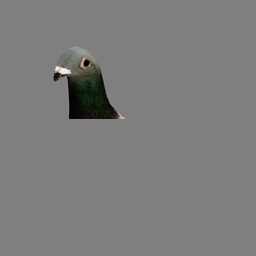
\includegraphics[width=0.20\linewidth]{figures/bird_crop_example.png}
    }
    \subfloat[Chair]{
        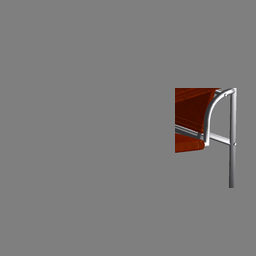
\includegraphics[width=0.20\linewidth]{figures/chair_crop_example.png}
    }
    \subfloat[Dog]{
        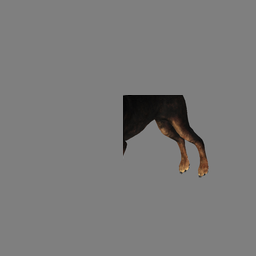
\includegraphics[width=0.20\linewidth]{figures/dog_crop_example.png}
    }
    \subfloat[Car]{
        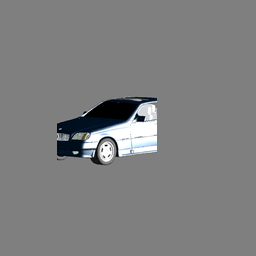
\includegraphics[width=0.20\linewidth]{figures/car_crop_example.png}
    }
    \caption{Examples of data augmentation on rendered images. For each image, everything except a section is hidden. By doing so, we introduce an \emph{attention} mechanism where the model can learn to associate sketches to particular details in the rendered image.}
    \label{fig:augment_example}
\end{figure}

\subsection*{Visual encoder specification}

The purpose of the visual encoder is to learn a function from images and sketches to a shared embedding space. The encoder network takes as input mid-level convolutional features from VGG-19. \change[JEF]{In our experiments, we used the fourth convolutional layer after the second pooling step.}{In our experiments, we used the second convolutional layer after the third pooling step.} \note[JEF] {Verify?} We chose a mid-convolutional layer to capitalize on successive layers of abstraction from early convolutional layers and to preserve two-dimensional structure. The encoder produces a shared embedding of size 1000. 

The architecture of the encoder is as follows: a single convolutional layer (conv1) with 64 filters, a kernel size of 3, a padding of 1, and a stride of 1; followed by a max pool layer with a stride of 2 and a dilation of 1; followed by two fully connected layers (fc1, fc2) to project to 4096 units and 1000 units, respectively. We include batch normalization and ReLU nonlinearity after conv1 and fc1. A dropout layer is added after fc1. We emphasize that the architecture of the encoder is purposefully chosen to be light weight. 

\subsection*{Visual encoder training procedure}

The dataset is split into training and testing based on the context, which is defined as the set of the target and distractor images (each trial consists of 3 distractor images and 1 target). The contexts of training examples will not overlap with the contexts of test examples. In practice, we have a 75\%, 25\% split ratio.

The binary classification task is to predict whether or not a given sketch is of a given image. Positive examples come from pariticipants' sketches and their corresponding target images. Negative samples come from pairing a participant's sketch with a randomly chosen image from the set of all images excluding the correct image. We note that training and testing sets will include examples from both close- and far-contexts. This training procedure closely resembles training Word2Vec with skip-gram and negative sampling where there is a similar motivation of learning shared embedding spaces.

During training, the model is shown minibatches of tuples, where each tuple contains $(r_{1}, s_{1})$, $(r_{2}, s_{2})$, $(r_{1}, s_{2})$, $(r_{2}, s_{1})$ where $r_{1}$, $r_{2}$ are two rendered images, and $(s_{1}, s_{2})$ are two sketches i.e. a minibatch of 10 would contain 40 examples. Each tuple is as follows: choose the next available image $r_{1}$, find its corresponding sketch $s_{1}$; choose 1 of the 3 distractor images from the same trial as $r_{2}$; its corresponding sketch is $s_{2}$. In each tuple, the first two examples are positive and last two examples are negative. The intuition behind this design is to balance the classes shown to the model at each gradient step.

Given an image $r_{i}$, a sketch $s_{i}$ and the label $l_{i}$, we define the objective function $J$ as 

\begin{multline}
    J(r_{i}, s_{i}) = -l_{i} \textup{ log}(\sigma(\textup{corr}(f(r_{i}), f(s_{i})))) \\ - (1 - l_{i}) \textup{ log}(1 - \sigma(\textup{corr}(f(r_{i}), f(s_{i}))))
\end{multline}

where $f$ is the visual encoder network, $\sigma$ is a sigmoid transformation, and $\textup{corr}$ is pearson correlation. We train the model using stochastic gradient descent via Adam with a learning rate of $0.001$, a batch size of $25$ for $20$ epochs. We use early stopping based on a small validation set. The trained model has 73.6\% classification accuracy on the held-out test set, suggesting some generalization to unseen contexts.

}

\showmatmethods{} % Display the Materials and Methods section

\acknow{Please include your acknowledgments here, set in a single paragraph. Please do not include any acknowledgments in the Supporting Information, or anywhere else in the manuscript.}

\showacknow{} % Display the acknowledgments section

% \pnasbreak splits and balances the columns before the references.
% Uncomment \pnasbreak to view the references in the PNAS-style
% If you see unexpected formatting errors, try commenting out \pnasbreak
% as it can run into problems with floats and footnotes on the final page.
%\pnasbreak

% Bibliography
\bibliography{references}

\end{document}
